\documentclass[main.tex]{subfiles}

\begin{document}

\section{Ecualización Adaptativa por Inversión de Sistemas}

El objetivo del proyecto es invertir los efectos del canal 
-el sistema desconocido- mediante el esquema de filtrado
adaptativo conocido como inversión de sistemas. El diagrama se muestra 
a continuación:

\begin{figure}[h]
    \centering
    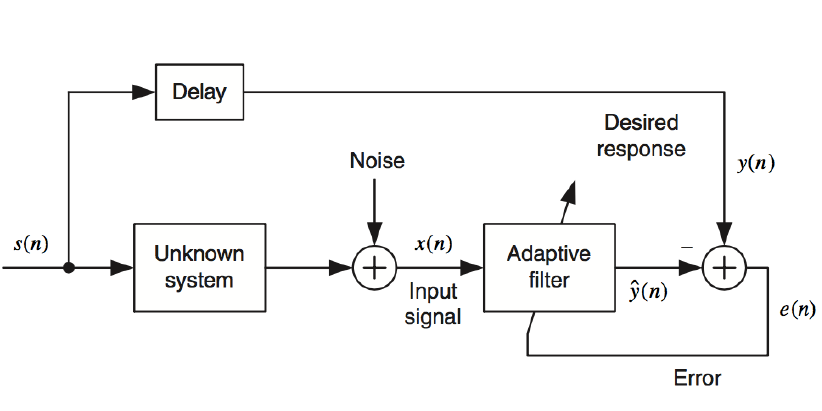
\includegraphics[scale=0.5]{imagenes/block.PNG}
    \caption{Inversión de sistemas.}
\end{figure}

En principio se asume que el ruido del canal 
es incorrelacionado con $s(n)$.\todo[inline]{cambiar nombres al esquema y al texto}
El filtrado funciona de la siguiente manera, se tiene 
la señal de entrada $s(n)$, que se transmite por el sistema
desconocido -el canal ya mencionado-, cuya salida es la señal 
$x(n)=u(n)$, que es la entrada al filtro adaptativo, de donde se obtiene
$\hat{y}(n)$. Realimentando la señal de error $e(n)$
al filtro adaptativo se maximiza la correlación entre la salida del 
filtro y la señal deseada $y(n)=d(n)$.
Opcionalmente, a su vez, se puede colocar un delay, retrasando la señal al obtener 
$d(n)$ para compensar el delay propio del sistema.\newline
Con ésto se consigue una salida con una respuesta en frecuencia inversa
al sistema desconocido, lo que anula su efecto.\newline
Sin embargo, en un enlace digital el receptor no conoce la respuesta deseada, por lo que
este esquema no es de utilidad. La solución consiste en utilizar 
una secuencia de entrenamiento, una respuesta deseada $d(n)$ preacordada entre 
emisor y receptor.
El diagrama de bloques completo se observa en la figura siguiente:
\begin{figure}[h]
    \centering
    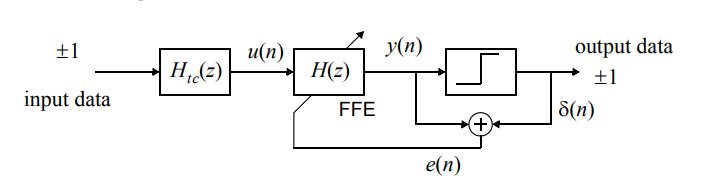
\includegraphics[scale=0.45]{imagenes/esquema.PNG}
    \caption{Diagrama de bloques con decision-directed feedback.}
\end{figure}
Luego del período de entrenamiento inicial los coeficientes del ecualizador pueden ser
 continuamente ajustados con un decision-directed feedback. De esta manera, 
 la señal de error $e(n)=d(n)-y(n)$ se deriva del último (no necesariamente correcto) 
 bit estimado de la secuencia transmitida $u(n)$. 
 
 En este caso, como la se\~nal se encontraba codificada en formato Manchester, la decisi\'on
 del bit recibido no consist\'ia en un simple comparador, sino que se utiliz\'o la regla de decisi\'on
 bayesiana \cite{shanmugan}. Partiendo de la regla:
 
 \begin{equation}
 	y^{T} \cdot (s_1 - s_0) \underset{H_0}{\overset{H_1}{\gtrless}} 
 	\sigma^2 \cdot \ln{\left( \frac{P(H_0)}{P(H_1)} \right)}
 	+ \frac{1}{2} \left( s_1^T s_1 - s_0^T s_0\right)
 \end{equation}
 
 donde $y$ es un vector con 16 mediciones, $s_1$ contiene las 16 muestras que forman un bit de 1 (es decir, 8 veces el valor -1 seguido de 8 veces el valor 1), y $s_0$, las que forman un 0. Como $s_0 = -s_1$, y ambos s\'imbolos son equiprobables (lo cual asumimos porque no conocemos a priori las caracter\'isticas del mensaje que se mandar\'a), la expresi\'on se ve simplificada en:
 
 \begin{equation}
 	y^{T} \cdot s_1 \underset{H_0}{\overset{H_1}{\gtrless}} 0
 \end{equation}
 
Considerando las caracter\'isticas de la codificaci\'on Manchester, la regla de decisi\'on resulta ser:

\begin{equation}
	\sum_{i=0}^7 y_i \underset{H_0}{\overset{H_1}{\lessgtr}}
	\sum_{i=8}^{15} y_i
\end{equation} 
 
\end{document}